\documentclass[journal,12pt,twocolumn]{IEEEtran}

\usepackage{setspace}
\usepackage{gensymb}
\singlespacing
\usepackage[cmex10]{amsmath}

\usepackage{amsthm}

\usepackage{mathrsfs}
\usepackage{txfonts}
\usepackage{stfloats}
\usepackage{bm}
\usepackage{cite}
\usepackage{cases}
\usepackage{subfig}

\usepackage{longtable}
\usepackage{multirow}

\usepackage{enumitem}
\usepackage{mathtools}
\usepackage{steinmetz}
\usepackage{tikz}
\usepackage{circuitikz}
\usepackage{verbatim}
\usepackage{tfrupee}
\usepackage[breaklinks=true]{hyperref}
\usepackage{graphicx}
\usepackage{tkz-euclide}
\usepackage{float}

\usetikzlibrary{calc,math}
\usepackage{listings}
    \usepackage{color}                                            %%
    \usepackage{array}                                            %%
    \usepackage{longtable}                                        %%
    \usepackage{calc}                                             %%
    \usepackage{multirow}                                         %%
    \usepackage{hhline}                                           %%
    \usepackage{ifthen}                                           %%
    \usepackage{lscape}     
\usepackage{multicol}
\usepackage{chngcntr}

\DeclareMathOperator*{\Res}{Res}

\renewcommand\thesection{\arabic{section}}
\renewcommand\thesubsection{\thesection.\arabic{subsection}}
\renewcommand\thesubsubsection{\thesubsection.\arabic{subsubsection}}

\renewcommand\thesectiondis{\arabic{section}}
\renewcommand\thesubsectiondis{\thesectiondis.\arabic{subsection}}
\renewcommand\thesubsubsectiondis{\thesubsectiondis.\arabic{subsubsection}}


\hyphenation{op-tical net-works semi-conduc-tor}
\def\inputGnumericTable{}                                 %%

\lstset{
%language=C,
frame=single, 
breaklines=true,
columns=fullflexible
}
\begin{document}

\newcommand{\BEQA}{\begin{eqnarray}}
\newcommand{\EEQA}{\end{eqnarray}}
\newcommand{\define}{\stackrel{\triangle}{=}}
\bibliographystyle{IEEEtran}
\raggedbottom
\setlength{\parindent}{0pt}
\providecommand{\mbf}{\mathbf}
\providecommand{\pr}[1]{\ensuremath{\Pr\left(#1\right)}}
\providecommand{\qfunc}[1]{\ensuremath{Q\left(#1\right)}}
\providecommand{\sbrak}[1]{\ensuremath{{}\left[#1\right]}}
\providecommand{\lsbrak}[1]{\ensuremath{{}\left[#1\right.}}
\providecommand{\rsbrak}[1]{\ensuremath{{}\left.#1\right]}}
\providecommand{\brak}[1]{\ensuremath{\left(#1\right)}}
\providecommand{\lbrak}[1]{\ensuremath{\left(#1\right.}}
\providecommand{\rbrak}[1]{\ensuremath{\left.#1\right)}}
\providecommand{\cbrak}[1]{\ensuremath{\left\{#1\right\}}}
\providecommand{\lcbrak}[1]{\ensuremath{\left\{#1\right.}}
\providecommand{\rcbrak}[1]{\ensuremath{\left.#1\right\}}}
\theoremstyle{remark}
\newtheorem{rem}{Remark}
\newcommand{\sgn}{\mathop{\mathrm{sgn}}}
\providecommand{\abs}[1]{\vert#1\vert}
\providecommand{\res}[1]{\Res\displaylimits_{#1}} 
\providecommand{\norm}[1]{\lVert#1\rVert}
%\providecommand{\norm}[1]{\lVert#1\rVert}
\providecommand{\mtx}[1]{\mathbf{#1}}
\providecommand{\mean}[1]{E[ #1 ]}
\providecommand{\fourier}{\overset{\mathcal{F}}{ \rightleftharpoons}}
%\providecommand{\hilbert}{\overset{\mathcal{H}}{ \rightleftharpoons}}
\providecommand{\system}{\overset{\mathcal{H}}{ \longleftrightarrow}}
	%\newcommand{\solution}[2]{\textbf{Solution:}{#1}}
\newcommand{\solution}{\noindent \textbf{Solution: }}
\newcommand{\cosec}{\,\text{cosec}\,}
\providecommand{\dec}[2]{\ensuremath{\overset{#1}{\underset{#2}{\gtrless}}}}
\newcommand{\myvec}[1]{\ensuremath{\begin{pmatrix}#1\end{pmatrix}}}
\newcommand{\mydet}[1]{\ensuremath{\begin{vmatrix}#1\end{vmatrix}}}
\numberwithin{equation}{subsection}
\makeatletter
\@addtoreset{figure}{problem}
\makeatother
\let\StandardTheFigure\thefigure
\let\vec\mathbf
\renewcommand{\thefigure}{\theproblem}
\def\putbox#1#2#3{\makebox[0in][l]{\makebox[#1][l]{}\raisebox{\baselineskip}[0in][0in]{\raisebox{#2}[0in][0in]{#3}}}}
     \def\rightbox#1{\makebox[0in][r]{#1}}
     \def\centbox#1{\makebox[0in]{#1}}
     \def\topbox#1{\raisebox{-\baselineskip}[0in][0in]{#1}}
     \def\midbox#1{\raisebox{-0.5\baselineskip}[0in][0in]{#1}}

\vspace{3cm}

\title{AI1103-Assignment 1}
\author{Name: Ramanathan Annamalai\\\normalsize{Roll Number: BM20BTECH11011\\\includegraphics[scale=0.34]{IITHLogo.png}}}
\maketitle
\newpage
\bigskip
\renewcommand{\thefigure}{\theenumi}
\renewcommand{\thetable}{\theenumi}
Download all python codes from 
\begin{lstlisting}
https://github.com/Ramanathan-Annamalai/AI1103-Probability_and_Random_Variables/tree/main/Assignment%201/Codes
\end{lstlisting}
%
and latex-tikz codes from 
%
\begin{lstlisting}
https://github.com/Ramanathan-Annamalai/AI1103-Probability_and_Random_Variables/blob/main/Assignment%201/Assignment_1.tex
\end{lstlisting}
\section*{Question}
Two cards are drawn successively with replacement from a well shuffled deck of 52 cards. Find the probability distribution of the number of aces.

\section*{Solution}
A deck of 52 cards contains 4 Aces i.e 1 from each suit.


Let probability of picking an ace from a well shuffled deck be \(p\)
\begin{align}
    p &= \frac{\text{No. of favourable cases}}{\text{Total no. of cases}}\nonumber\\
    &=\frac{4}{52} = \frac{1}{13}\\\nonumber
\end{align}

Probability of not picking an ace from the deck will be represented by \(q\)
\begin{align}
    q&=(1-p)\nonumber\\
    &=\frac{48}{52} = \frac{12}{13}\\\nonumber
\end{align}

We are drawing two card from the deck, with replacement. Let \(X \in \{0,1,2\}\) represent the random variable, where
\begin{enumerate}
    \item 0 represents drawing no aces
    \item 1 represents drawing one ace
    \item 2 represents drawing two aces
\end{enumerate}
\section*{}
Now, let us find the probability distribution:
\begin{enumerate}
    \item Drawing no aces:
    \begin{align}
        Pr(X=0) = q \times q &= q^2\\
        &= \frac{144}{169}\\\nonumber
    \end{align}
    \item Drawing one ace:
    \begin{align}
        Pr(X=1) &= p \times q + q \times p\\
        &= 2pq = \frac{24}{169}\\\nonumber
    \end{align}
    \item Drawing both aces:
    \begin{align}
        Pr(X=2) = p \times p &= p^2\\
        &= \frac{1}{169}\\\nonumber
    \end{align}
\end{enumerate}

\begin{table}[H]
    \centering
        \begin{tabular}{|c|r|}
            \hline
            \multirow{2}{*}{\normalsize{Random Variable [X]}} &   \multirow{2}{*}{\normalsize{Probability [Pr(X)}}    \\
                                        &                                                \\\hline
            \multirow{2}{*}{\large{0}}  &   \multirow{2}{*}{\large{\(q^2 = \frac{144}{169}\)}} \\
                                        &                                                \\\hline
            \multirow{2}{*}{\large{1}}  &   \multirow{2}{*}{\large{\(2pq = \frac{24}{169}\)}}  \\
                                        &                                                \\\hline
            \multirow{2}{*}{\large{2}}  &   \multirow{2}{*}{\large{\(p^2 = \frac{1}{169}\)}}   \\
                                        &                                                \\\hline
    \end{tabular}
    \caption{Probability distribution values for the outcomes of the event.}
    \label{Probabilty Distribution Table}
\end{table}

\begin{figure}[H]
    \centering
    \frame{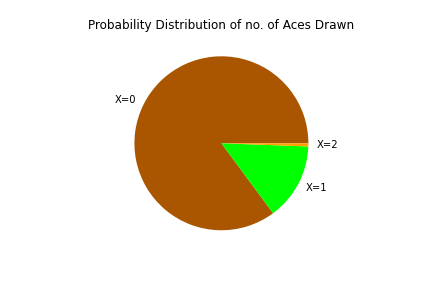
\includegraphics[width=\linewidth]{Pie_chart.png}}
    \caption{Representation of Theory}
    \label{Pie chart}
\end{figure}

\begin{figure}[H]
    \centering
    \frame{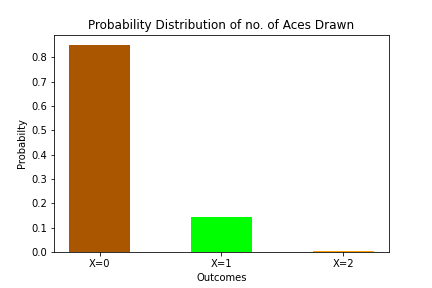
\includegraphics[width=\linewidth]{Bar_graph.png}}
    \caption{Theory vs Simulation}
    \label{Bar Chart}
\end{figure}

\end{document}
